% !TeX encoding = UTF-8
% !TeX program = xelatex
\documentclass[12pt, a4paper]{article}
\usepackage{xeCJK} % 须放在\usepackage{}列中足够前的位置
\usepackage{fontspec}
\usepackage{graphicx}
\usepackage{caption}
\usepackage{enumerate}
\usepackage{setspace}
\usepackage{array} % 製作表格必須的宏包
\usepackage{tabularx} % 自動調整列寬的表格宏包
\usepackage{adjustbox}
\setCJKfamilyfont{heiti}{Heiti TC}
\CJKfamily{heiti}
\setmainfont{Arial}
\setstretch{1.5}


\begin{document}
\begin{center}
  {\Huge 邏輯設計實驗} \\[2.5cm]
  {\Huge Lab14} \\[1.5cm]
  {\Huge 有限狀態機} \\ [4.5cm]
  \hspace{.6in}
  \begin{minipage}[t]{.4\linewidth}
    {\Large 班級:資訊一甲}\\[0.5cm]
    {\Large 學號:D1109023}\\[0.5cm]
    {\Large 姓名:楊孟憲}
  \end{minipage}    
\end{center}

\newpage

\begin{description}
  \fontsize{22pt}{25pt}\selectfont 
    \item [一、]摘要 
      \begin{enumerate}
        \fontsize{20pt}{22pt}\selectfont
          \item 有限狀態機設計步驟 
            \fontsize{16pt}{20}\selectfont
              \begin{description}
                \item [$(1)$] 觀察狀態圖
                \item [$(2)$] 依據狀態圖,繪製狀態表 
                \item [$(3)$] 狀態簡化
                \item [$(4)$] 狀態變數指定
                \item [$(5)$] 配合正反器之激勵表,推導轉態表
                \item [$(6)$] 利用卡諾圖化簡正反器輸入的最簡布林代數
                \item [$(7)$] 根據布林代數繪出序向邏輯電路
                \bf 狀態表
                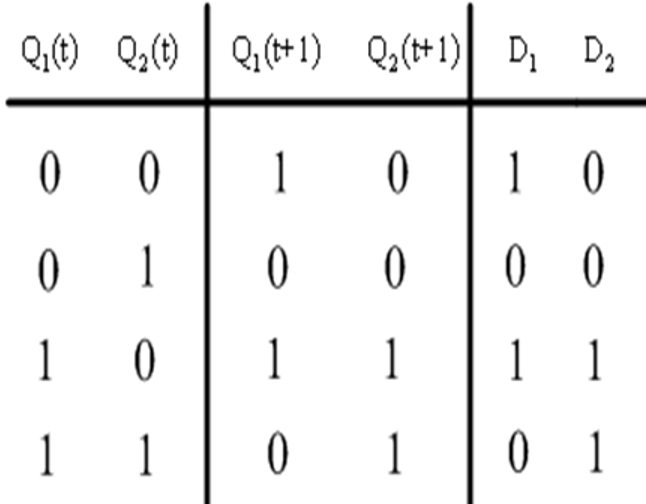
\includegraphics[width=10cm]{./image/designed-the-kmap.png}
              \end{description}

          \fontsize{20pt}{22}\selectfont 
          \item 實驗 
            \begin{description}
              \fontsize{16pt}{20}\selectfont
                \item [(1)] 使用3個D正反器設計一個學號產生器 
                \item [(2)] 使用3個D正反器設計一個順時鐘閃爍的跑馬燈 \\
              \normalsize  
            \end{description}
        \normalsize
      \end{enumerate}

    \item [二、]實驗結果
      \begin{description}
        \fontsize{20pt}{22pt}\selectfont
        \item 實驗一 \space{1em}使用3個D正反器設計一個學號產生器
            \begin{description}
              \fontsize{18pt}{20pt}
                \item [$\bullet$] CLK 頻率為 1 Hz 
                \item [$\bullet$] 本計數器為 Moore Machine \\
                \item []電路圖 \\[.3cm]
                  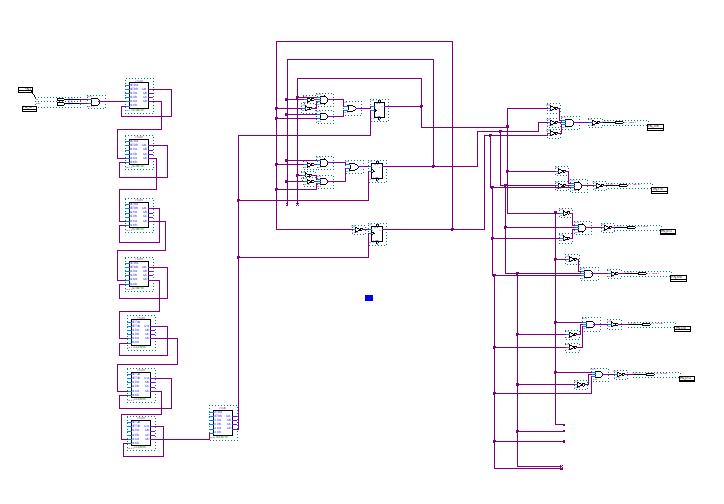
\includegraphics[width=13cm]{./image/ex1.png}
            \end{description}
          \normalsize
          
          \fontsize{20pt}{22pt}\selectfont
          \item 實驗二 \space 使用3個D正反器設計一個順時鐘閃爍的跑馬燈 \\
            \fontsize{16pt}{18pt}\selectfont
              \begin{description}
                \item [$\bullet$] CLK 頻率為 1 Hz
                \item [$\bullet$] Start=0, 停止閃爍, Start=1, 開始閃爍
                \fontsize{18pt}{20pt}
                  \item []電路圖 \\[.3cm]
                    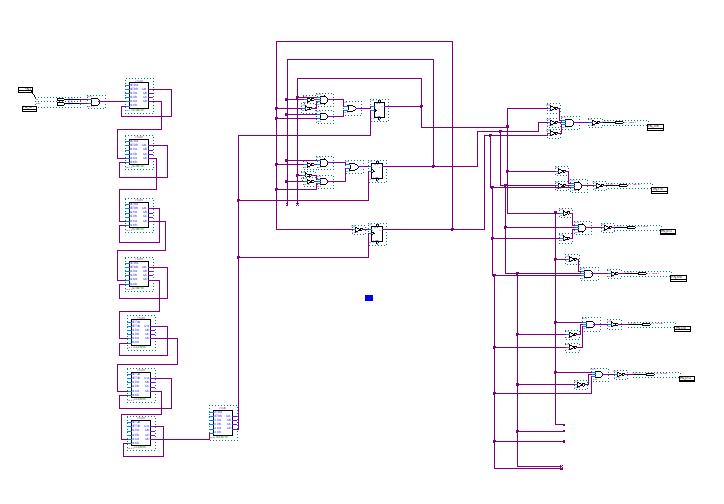
\includegraphics[width=13cm]{./image/ex2.png}
              \end{description}
            \normalsize
        \normalsize
      \end{description}
    \item [三]問題討論心得 \\[.6cm]
      \begin{minipage}[t]{\linewidth}
        \fontsize{16}{18}\selectfont
        本次實驗是本最後一個實驗,也是我覺得最好玩的一次實驗。在上課之前對於本次的實驗想法截然不同,努力地找出規律並設計電路,但是經過老師講解的觀察狀態圖,在設計電路的技巧讓我大開眼界。這次實驗除了使用本學期教的 D-flip-flop 正反器,也需要透過觀察狀態圖並實際操作 k-map 後得到邏輯電路圖,接著再把電路接出,而這次的兩個實驗又有除頻器,讓我更加了解除頻器的操作原裡。 
      \end{minipage}
  \normalsize
\end{description}`

\end{document}


